\PassOptionsToPackage{unicode=true}{hyperref} % options for packages loaded elsewhere
\PassOptionsToPackage{hyphens}{url}
%
\documentclass[ignorenonframetext,]{beamer}
\usepackage{pgfpages}
\setbeamertemplate{caption}[numbered]
\setbeamertemplate{caption label separator}{: }
\setbeamercolor{caption name}{fg=normal text.fg}
\beamertemplatenavigationsymbolsempty
% Prevent slide breaks in the middle of a paragraph:
\widowpenalties 1 10000
\raggedbottom
\setbeamertemplate{part page}{
\centering
\begin{beamercolorbox}[sep=16pt,center]{part title}
  \usebeamerfont{part title}\insertpart\par
\end{beamercolorbox}
}
\setbeamertemplate{section page}{
\centering
\begin{beamercolorbox}[sep=12pt,center]{part title}
  \usebeamerfont{section title}\insertsection\par
\end{beamercolorbox}
}
\setbeamertemplate{subsection page}{
\centering
\begin{beamercolorbox}[sep=8pt,center]{part title}
  \usebeamerfont{subsection title}\insertsubsection\par
\end{beamercolorbox}
}
\AtBeginPart{
  \frame{\partpage}
}
\AtBeginSection{
  \ifbibliography
  \else
    \frame{\sectionpage}
  \fi
}
\AtBeginSubsection{
  \frame{\subsectionpage}
}
\usepackage{lmodern}
\usepackage{amssymb,amsmath}
\usepackage{ifxetex,ifluatex}
\usepackage{fixltx2e} % provides \textsubscript
\ifnum 0\ifxetex 1\fi\ifluatex 1\fi=0 % if pdftex
  \usepackage[T1]{fontenc}
  \usepackage[utf8]{inputenc}
  \usepackage{textcomp} % provides euro and other symbols
\else % if luatex or xelatex
  \usepackage{unicode-math}
  \defaultfontfeatures{Ligatures=TeX,Scale=MatchLowercase}
\fi
\usetheme[]{Dresden}
\usefonttheme{professionalfonts}
% use upquote if available, for straight quotes in verbatim environments
\IfFileExists{upquote.sty}{\usepackage{upquote}}{}
% use microtype if available
\IfFileExists{microtype.sty}{%
\usepackage[]{microtype}
\UseMicrotypeSet[protrusion]{basicmath} % disable protrusion for tt fonts
}{}
\IfFileExists{parskip.sty}{%
\usepackage{parskip}
}{% else
\setlength{\parindent}{0pt}
\setlength{\parskip}{6pt plus 2pt minus 1pt}
}
\usepackage{hyperref}
\hypersetup{
            pdftitle={Graph traversal and Path-finding Algorithms used in Video Games},
            pdfauthor={Marius Rabenarivo},
            pdfborder={0 0 0},
            breaklinks=true}
\urlstyle{same}  % don't use monospace font for urls
\newif\ifbibliography
\usepackage{graphicx,grffile}
\makeatletter
\def\maxwidth{\ifdim\Gin@nat@width>\linewidth\linewidth\else\Gin@nat@width\fi}
\def\maxheight{\ifdim\Gin@nat@height>\textheight\textheight\else\Gin@nat@height\fi}
\makeatother
% Scale images if necessary, so that they will not overflow the page
% margins by default, and it is still possible to overwrite the defaults
% using explicit options in \includegraphics[width, height, ...]{}
\setkeys{Gin}{width=\maxwidth,height=\maxheight,keepaspectratio}
\setlength{\emergencystretch}{3em}  % prevent overfull lines
\providecommand{\tightlist}{%
  \setlength{\itemsep}{0pt}\setlength{\parskip}{0pt}}
\setcounter{secnumdepth}{0}

% set default figure placement to htbp
\makeatletter
\def\fps@figure{htbp}
\makeatother


\title{Graph traversal and Path-finding Algorithms used in Video Games}
\author{Marius Rabenarivo}
\date{16th June 2024}
\titlegraphic{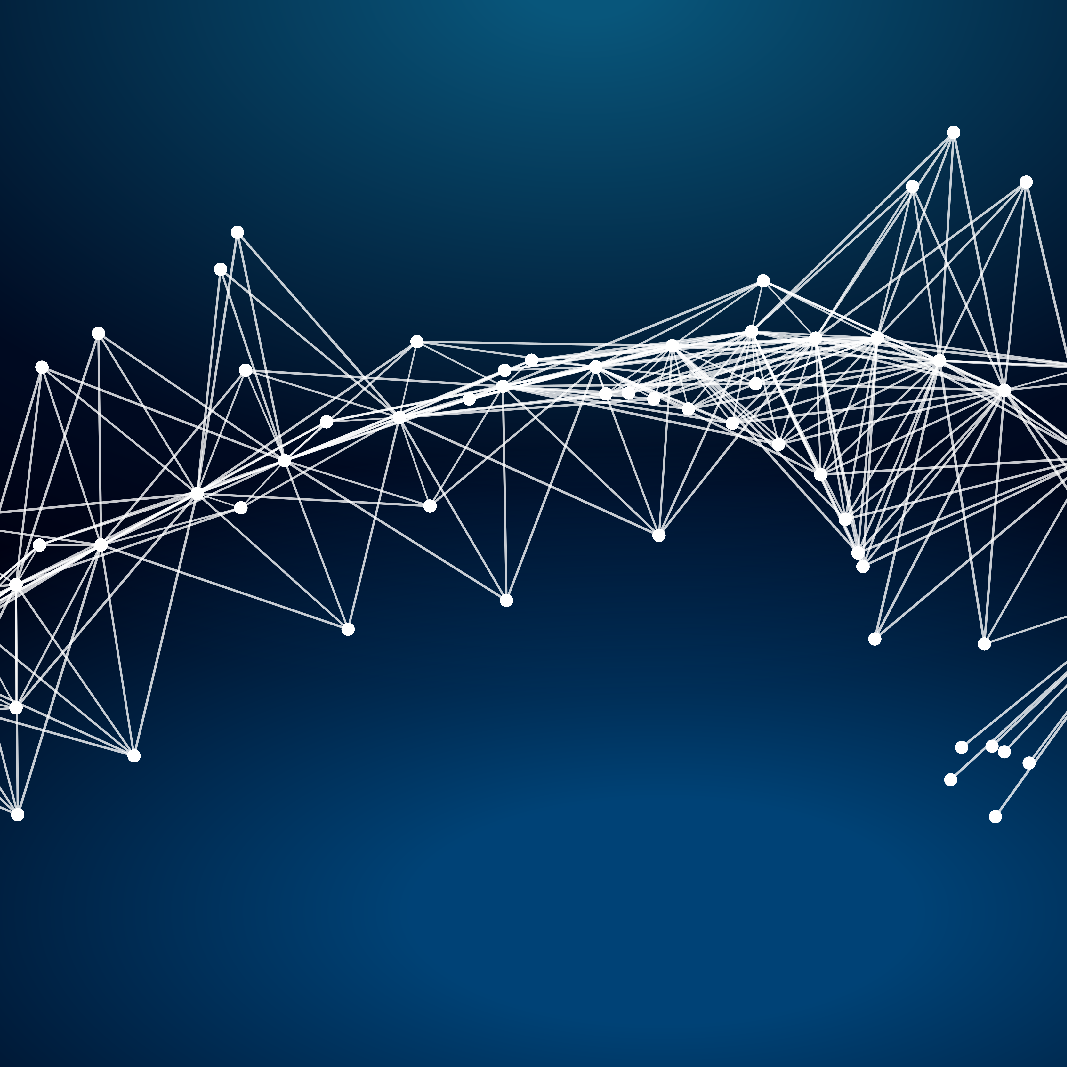
\includegraphics{background-graph.png}}
\logo{
\includegraphics{logo.png}}

\begin{document}
\frame{\titlepage}

\begin{frame}

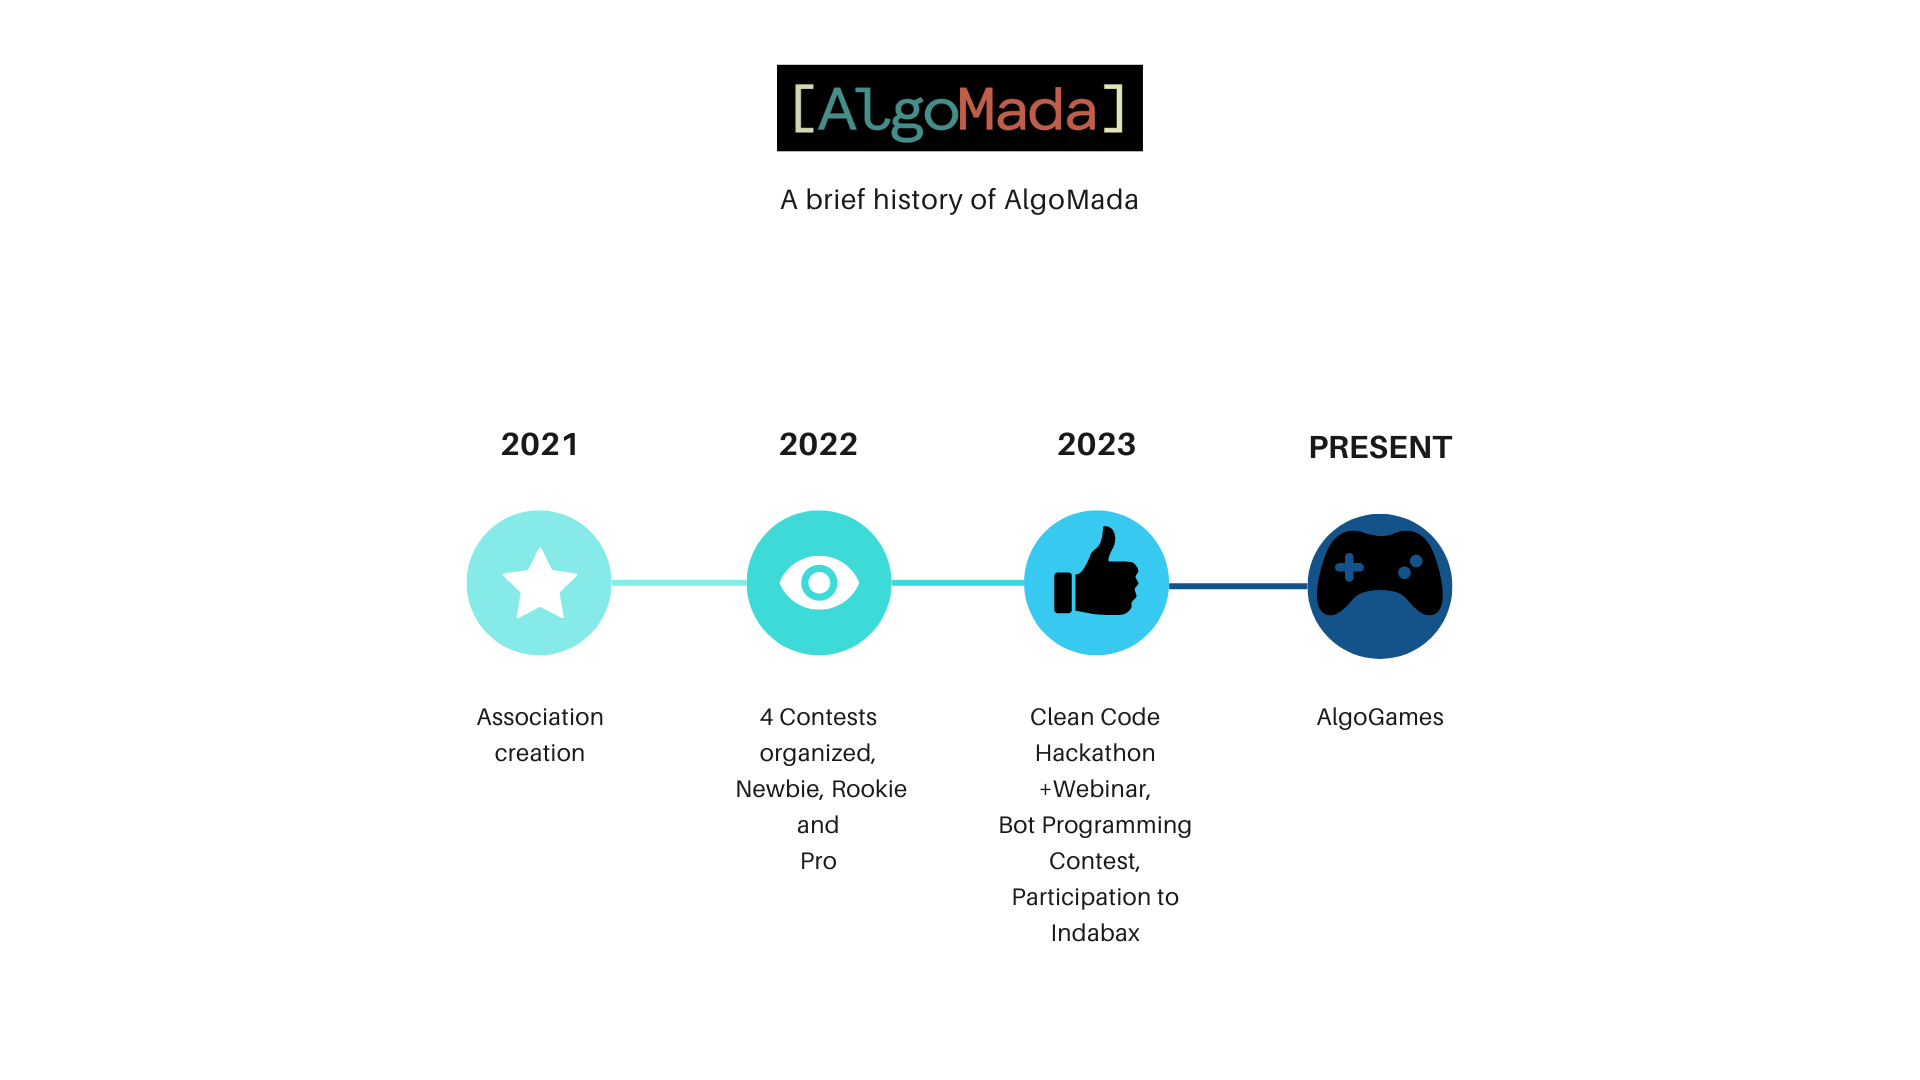
\includegraphics{AlgoMada.png}

\end{frame}

\begin{frame}{About me}
\protect\hypertarget{about-me}{}

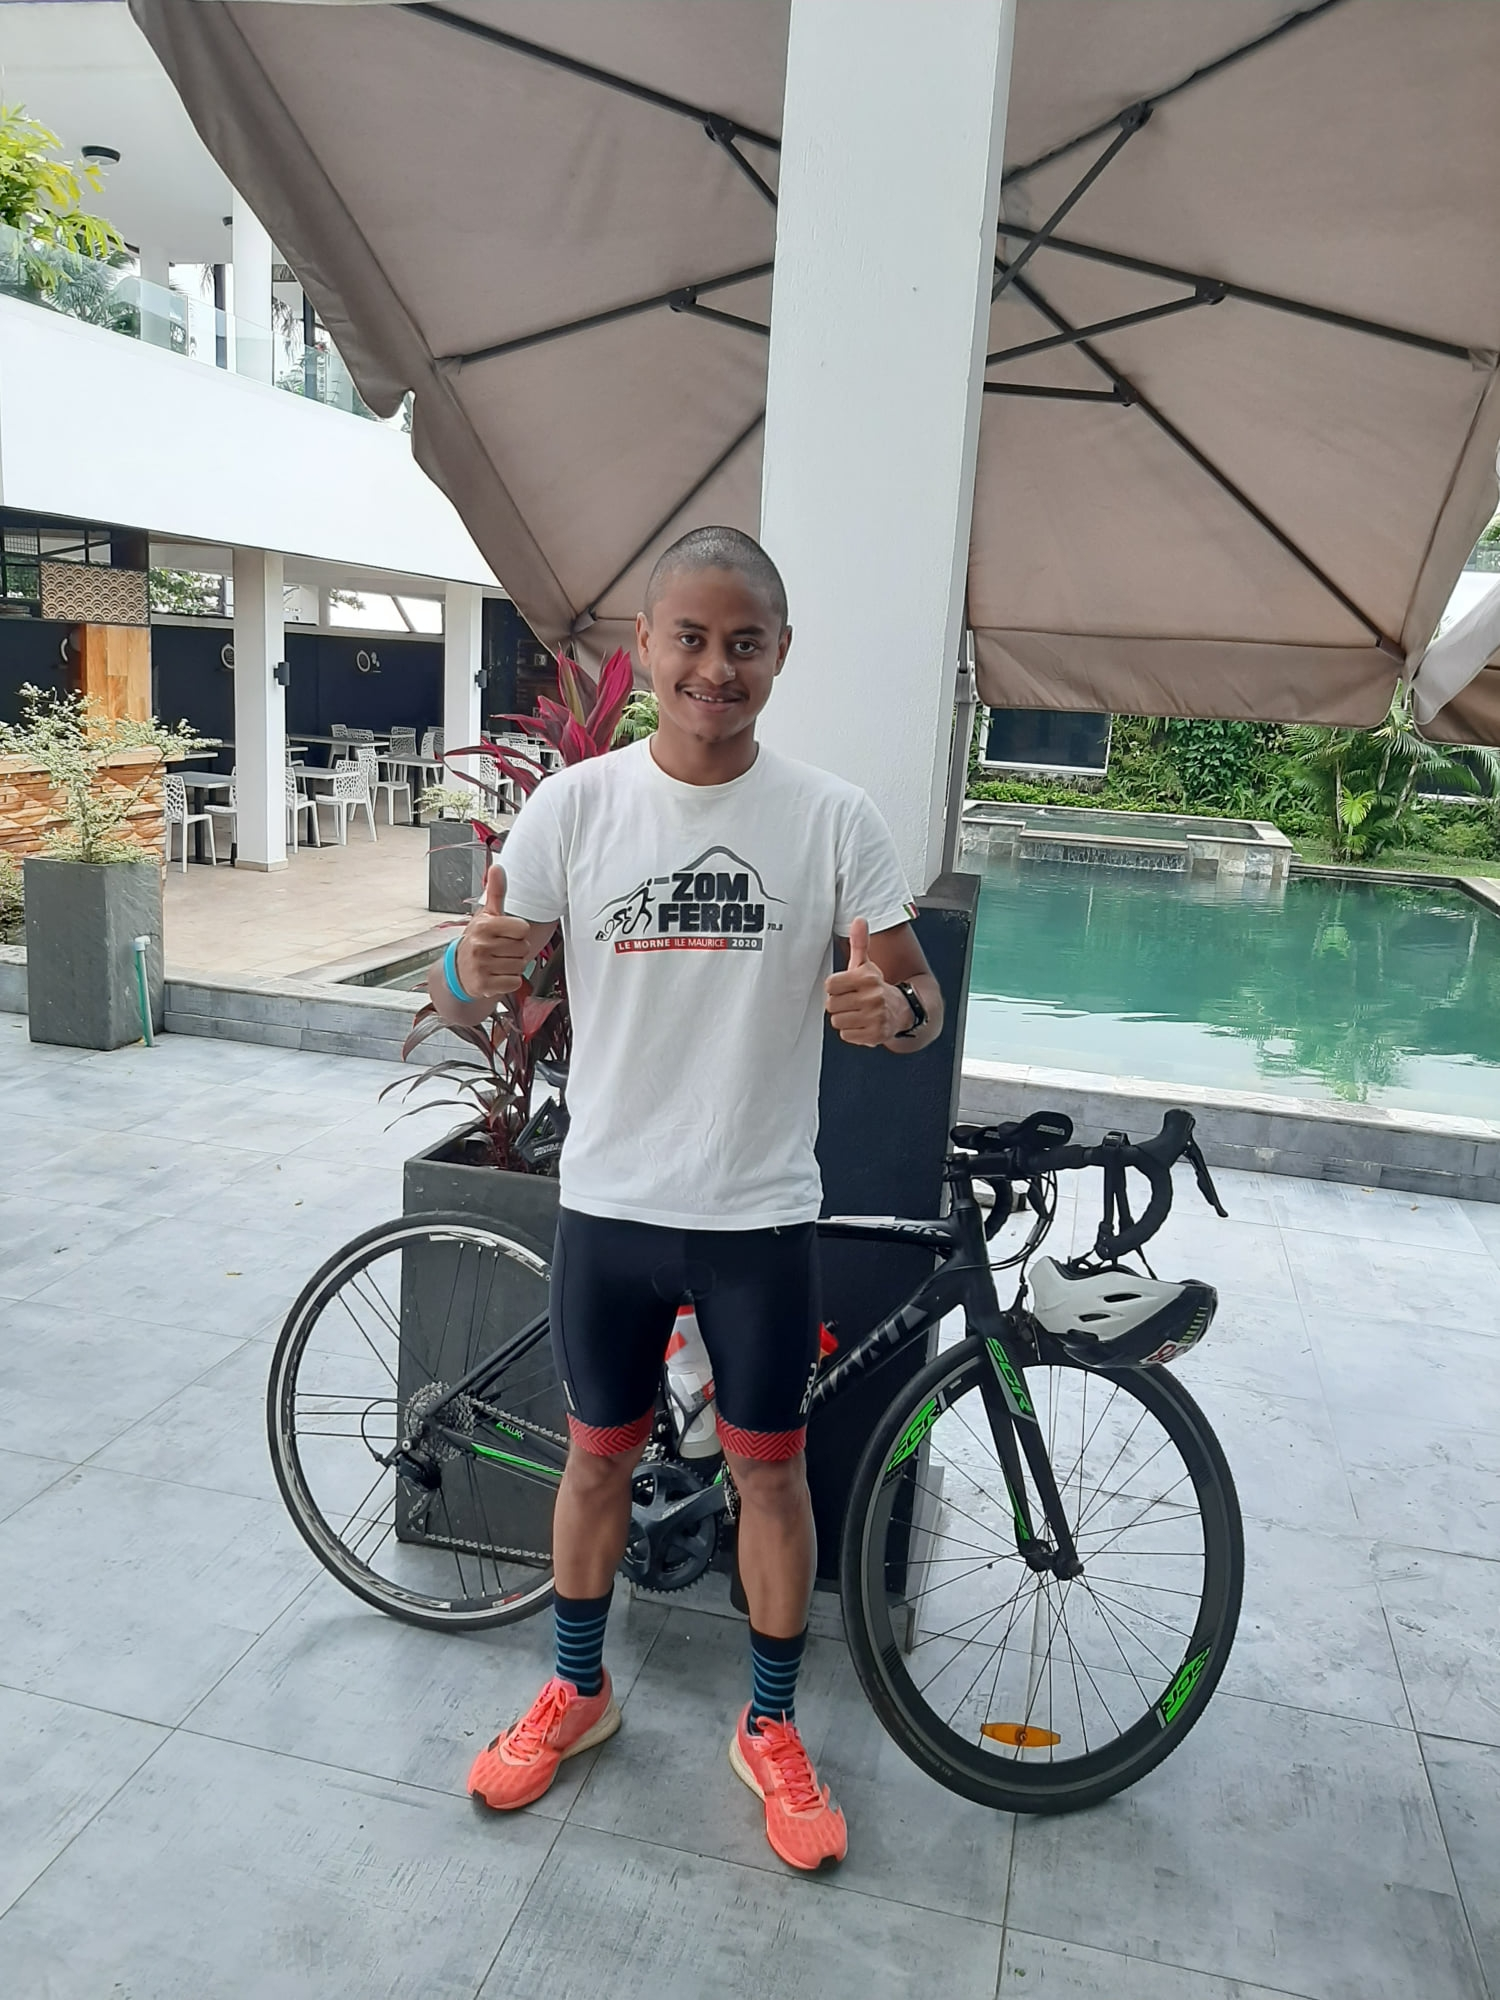
\includegraphics[width=\textwidth,height=1.04167in]{marius.jpg}

\begin{itemize}
\tightlist
\item
  Telecommunications, ESPA Alumni
\item
  Computer Science, University of Reunion Island Alumni
\item
  FaceDev Admin since 2012
\item
  Founder member of AlgoMada
\item
  Clojure dev
\item
  Computer Science Enthusiast
\item
  Current interests: Cryptocurrency, Clojure programming language
\item
  Side project: BetaX Community
\end{itemize}

\end{frame}

\begin{frame}{Motivation: Why I do this?}
\protect\hypertarget{motivation-why-i-do-this}{}

\begin{figure}
\centering
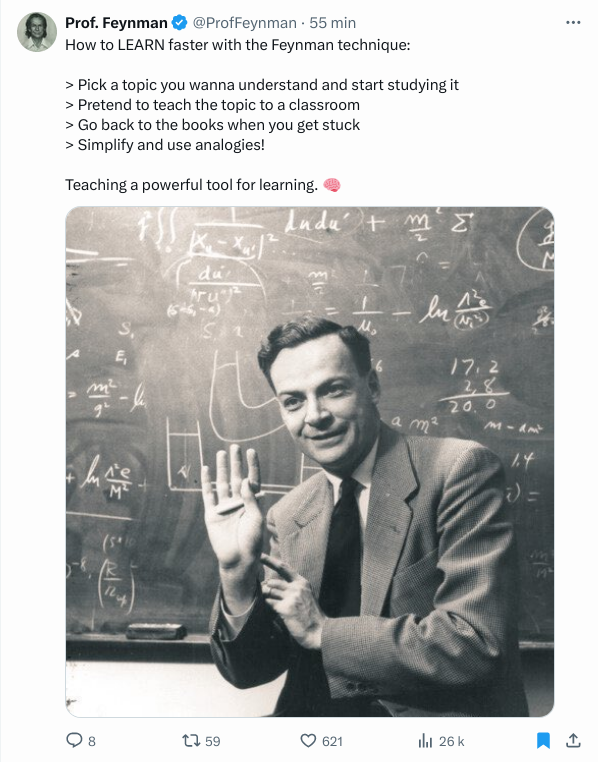
\includegraphics[width=\textwidth,height=2.34375in]{feynman-technique.png}
\caption{Feynman technique for studying}
\end{figure}

\end{frame}

\begin{frame}{Definition of Computer Science}
\protect\hypertarget{definition-of-computer-science}{}

``We are about to study the idea of a computational process.
Computational processes are abstract beings that inhabit computers. As
they evolve, processes manipulate other abstract things called data. The
evolution of a process is directed by a pattern of rules called a
program. People create programs to direct processes. In effect, we
conjure the spirits of the computer with our spells.'' Structure and
Interpretation of Computer Programs, Harold Abelson and Gerald J.
Sussman


\includegraphics[width=\textwidth,height=1.04167in]{Fujiwara_No_Mokou_Law_Is_SICP.png}

\end{frame}

\begin{frame}{What is a graph?}
\protect\hypertarget{what-is-a-graph}{}

A data structure to represent link between objects. A graph is defined
by a set of nodes V and a set of edges E.

We can summarize this definition by the following formula:

\[
G = (E, V)
\]

Example:
\url{https://www.redblobgames.com/pathfinding/grids/graphs.html\#properties}

\end{frame}

\begin{frame}{What's the difference between a graph and a tree?}
\protect\hypertarget{whats-the-difference-between-a-graph-and-a-tree}{}

A graph can contain cycles (a node can be visited twice).

\begin{figure}
\centering
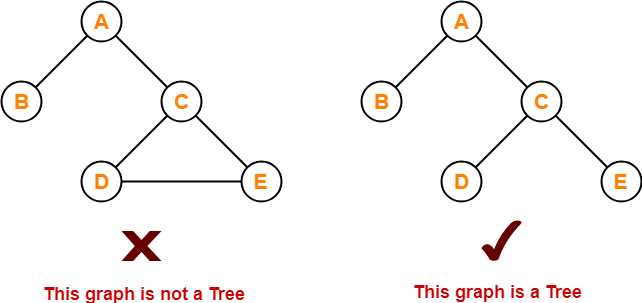
\includegraphics[width=\textwidth,height=2.08333in]{Tree-Data-Structure-Example.png}
\caption{Tree vs Graph}
\end{figure}

\end{frame}

\begin{frame}{Different type of graphs}
\protect\hypertarget{different-type-of-graphs}{}

\begin{itemize}
\tightlist
\item
  Acyclic Graph
\end{itemize}

A graph that has no cycle.

\begin{itemize}
\tightlist
\item
  Cyclic Graph
\end{itemize}

A graph that has at least one cycle.

\begin{figure}
\centering
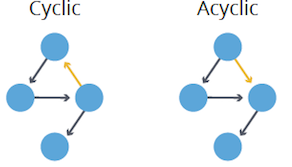
\includegraphics[width=\textwidth,height=1in]{acyclic-cyclic.png}
\caption{Acyclic vs Cyclic graph}
\end{figure}

\end{frame}

\begin{frame}{Different type of graphs}
\protect\hypertarget{different-type-of-graphs-1}{}

\begin{itemize}
\tightlist
\item
  Directed Graph
\end{itemize}

A graph in which edge has direction. That is the nodes are ordered pairs
in the definition of every edge.

\begin{itemize}
\tightlist
\item
  Undirected Graph
\end{itemize}

A graph in which edge are not directed. Meaning, the edges are defined
by an unordered pair of nodes.

\begin{figure}
\centering
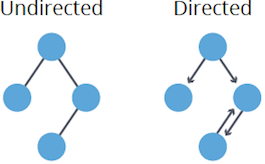
\includegraphics[width=\textwidth,height=1in]{undirected-directed.png}
\caption{Undirected vs Directed Graph}
\end{figure}

\end{frame}

\begin{frame}{Different type of graphs}
\protect\hypertarget{different-type-of-graphs-2}{}

\begin{itemize}
\tightlist
\item
  Directed Acyclic Graph
\end{itemize}

A graph that is both directed and acyclic.

\begin{figure}
\centering
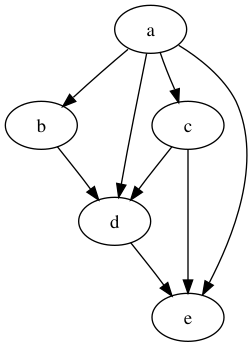
\includegraphics[width=\textwidth,height=1.82292in]{dag.png}
\caption{Directed Acyclic Graph}
\end{figure}

\end{frame}

\begin{frame}{Different type of graphs}
\protect\hypertarget{different-type-of-graphs-3}{}

\begin{itemize}
\tightlist
\item
  Connected graph
\end{itemize}

Every pair of nodes has a path linking them. Put in another way, there
are no inaccessible node.

\begin{itemize}
\tightlist
\item
  Disconnected graph
\end{itemize}

A graph in which there is at least one inaccessible node.

\begin{figure}
\centering
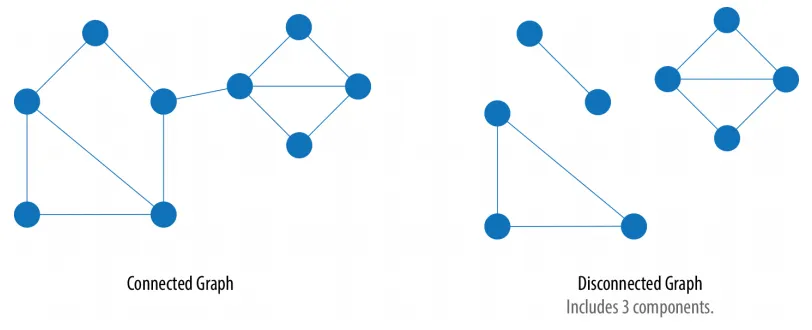
\includegraphics[width=\textwidth,height=1.04167in]{disconnected-connected.png}
\caption{Disconnected vs Connected Graph}
\end{figure}

\end{frame}

\begin{frame}{Different type of graphs}
\protect\hypertarget{different-type-of-graphs-4}{}

\begin{itemize}
\tightlist
\item
  A multigraph
\end{itemize}

A graph that can have multiple edges between the same nodes.

\begin{figure}
\centering
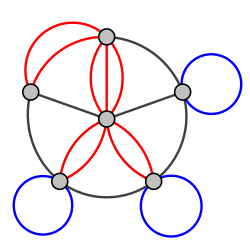
\includegraphics[width=\textwidth,height=1.5625in]{Multi-pseudograph.png}
\caption{A multigraph with multiple edges (red) and several loops
(blue). By 0x24a537r9 - Own work, CC BY-SA 3.0,
https://commons.wikimedia.org/w/index.php?curid=12247695}
\end{figure}

\end{frame}

\begin{frame}{Different way to represent a graph}
\protect\hypertarget{different-way-to-represent-a-graph}{}

There are 2 ways to represent a graph:

\begin{itemize}
\tightlist
\item
  adjacency list For each node, provide a list of other nodes that are
  adjacent to it.
\item
  adjacency matrix A matrix construct by aligning the nodes in the row
  and the columns and putting a value if the nodes are linked by an
  edge.
\end{itemize}

\begin{figure}
\centering
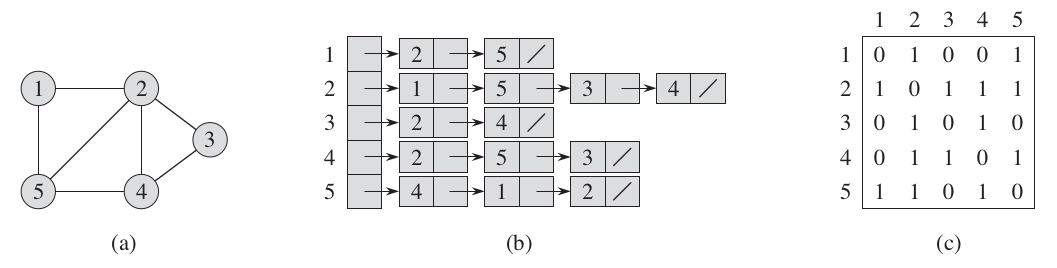
\includegraphics{graph-representation.png}
\caption{(a) Undirected graph with 5 vertices and 7 edges (b)
Adjacency-list representation (c) Adjacency-matrix representation}
\end{figure}

\end{frame}

\begin{frame}{Graph traversal algorithms}
\protect\hypertarget{graph-traversal-algorithms}{}

\begin{block}{BFS (Breadth-First Search)}

A graph traversal algorithm in which one explore every possible node in
the current depth level before going to the next. Usually used to find
shortest path distance from the start to a given vertex and the
associated predecessor subgraph.

\end{block}

\begin{block}{DFS (Depth-First Search)}

A graph traversal algorithm in which one start with a root node
(arbitrarily chosen) then explore as far as possible along each branch
before backtracking. Usually used as a subroutine in another algorithm.

\begin{figure}
\centering
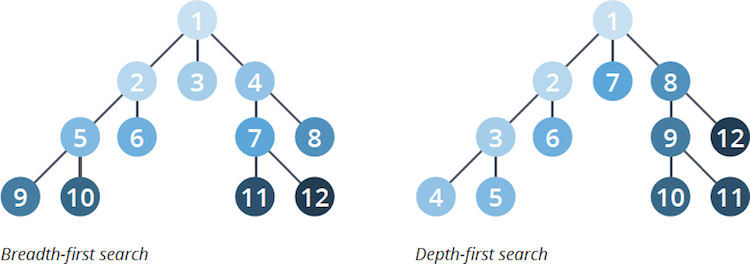
\includegraphics[width=\textwidth,height=0.83333in]{graph-traversal-algorithms-1.png}
\caption{Graph traversal algorithms}
\end{figure}

\end{block}

\end{frame}

\begin{frame}{BFS (Breadth-First Search)}
\protect\hypertarget{bfs-breadth-first-search-1}{}

\begin{figure}
\centering
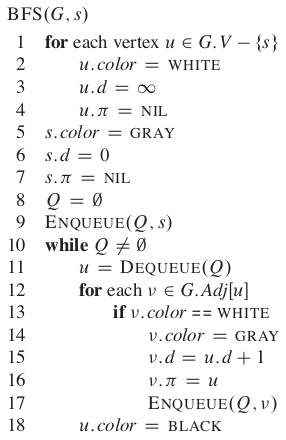
\includegraphics[width=\textwidth,height=2.34375in]{breadth-first-search-pseudocode.png}
\caption{Breadth-first search pseudo-code}
\end{figure}

\end{frame}

\begin{frame}{BFS (Breadth-First Search)}
\protect\hypertarget{bfs-breadth-first-search-2}{}

\begin{figure}
\centering
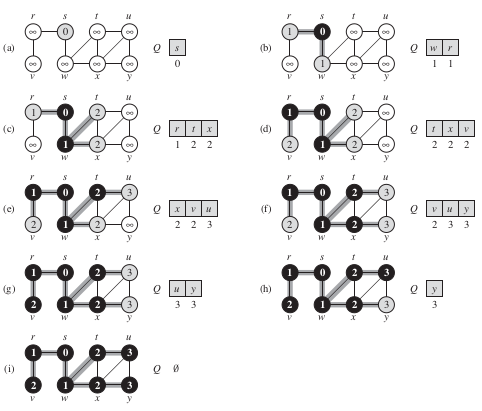
\includegraphics[width=\textwidth,height=2.34375in]{bfs-undirected-graph.png}
\caption{Operation of BFS on an undirected graph}
\end{figure}

\end{frame}

\begin{frame}{Predecessor subgraph}
\protect\hypertarget{predecessor-subgraph}{}

The procedure BFS builds a breadth-first tree as it searches the graph,
as Fig-11 illustrates. The tree corresponds to the \(\pi\) attributes.

More formally, for a graph \(G = (V, E)\) with source \(s\), we define
the \textbf{predecessor subgraph} of \(G\) as
\(G_{\pi} = (V_{\pi}, E_{\pi})\) \[
V_{\pi} = { v \in V : v.\pi \ne NIL }
\]

and

\[
E_{\pi} = { (v, \pi, v) : v \in V_{\pi} - {s} }
\]

\end{frame}

\begin{frame}{Breadth-first trees}
\protect\hypertarget{breadth-first-trees}{}

The predecessor subgraph \(G_{\pi}\) is a \textbf{breadth-first tree} if
\(V_{\pi}\) consists of the vertices reachable from \(s\) and, for all
\(v \in V\), the subgraph \(G_{\pi}\) contains a unique simple path from
\(s\) to \(v\) that is also a shortest path from \(s\) to \(v\) in
\(G\).

\end{frame}

\begin{frame}{Depth-First Search}
\protect\hypertarget{depth-first-search}{}

\begin{figure}
\centering
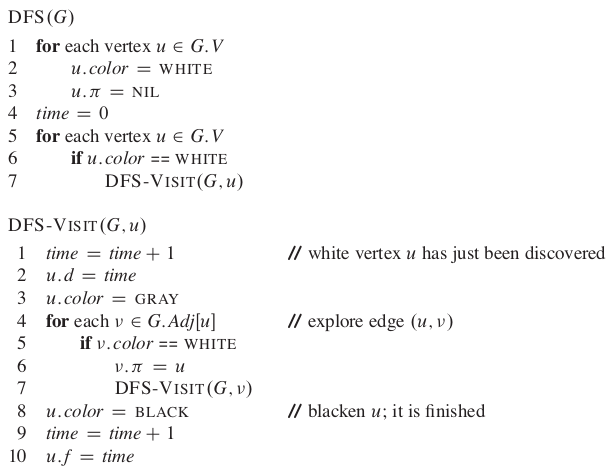
\includegraphics[width=\textwidth,height=2.34375in]{depth-first-search-pseudocode.png}
\caption{Depth-First Search Pseudocode}
\end{figure}

\end{frame}

\begin{frame}{Depth-First Search}
\protect\hypertarget{depth-first-search-1}{}

\begin{figure}
\centering
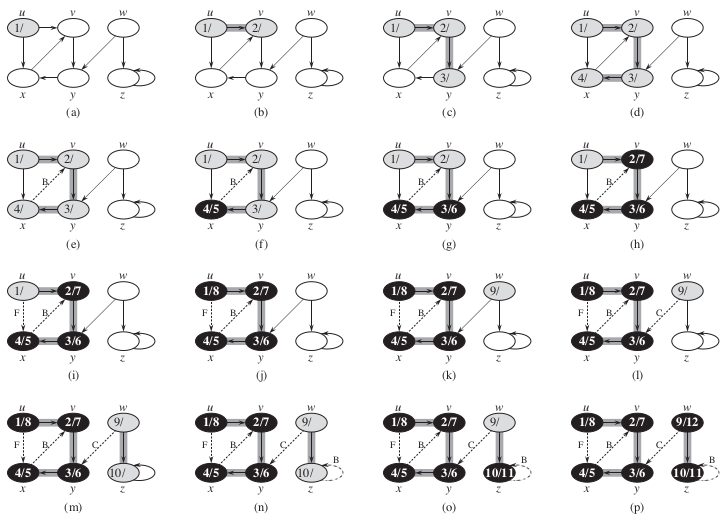
\includegraphics[width=\textwidth,height=2.34375in]{progress-dfs-directed-graph.png}
\caption{Depth-First Search progress on a directed graph}
\end{figure}

\end{frame}

\begin{frame}{Path finding algorithms}
\protect\hypertarget{path-finding-algorithms}{}

\begin{block}{A* algorithm}

A* (pronounced ``A-Star'') is a graph traversal and path-finding
algorithm. Given a source and a goal node, the algorithm find the
shortest-path (with respect to given weights) from source to goal.

\end{block}

\begin{block}{Dijkstra algorithm}

Dijkstra algorithm solves the single-source shortest-paths problem on a
weighted directed graph for the case in which all weights are
non-negative.

\end{block}

\end{frame}

\begin{frame}{Path-finding}
\protect\hypertarget{path-finding}{}

\begin{figure}
\centering
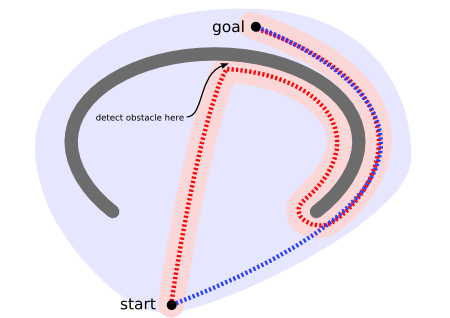
\includegraphics[width=\textwidth,height=2.34375in]{concave1.png}
\caption{Example path-finding situation}
\end{figure}

\end{frame}

\begin{frame}{Path-finding}
\protect\hypertarget{path-finding-1}{}

\begin{figure}
\centering
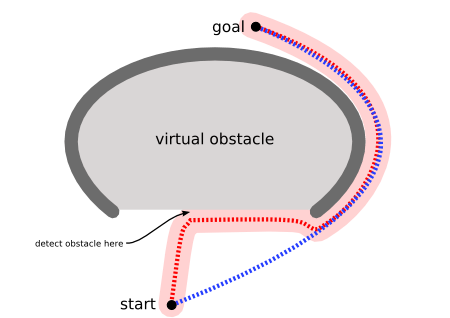
\includegraphics[width=\textwidth,height=2.34375in]{concave2.png}
\caption{Example path-finding situation}
\end{figure}

\end{frame}

\begin{frame}{A* Algorithm}
\protect\hypertarget{a-algorithm-1}{}

\begin{block}{History}

\begin{figure}
\centering
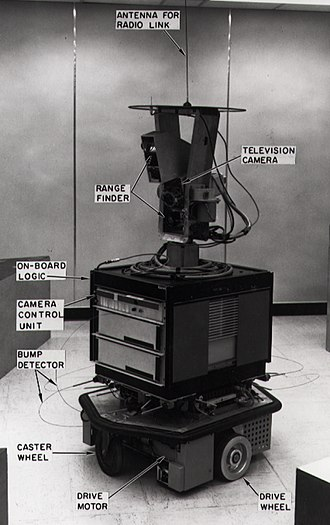
\includegraphics[width=\textwidth,height=2.08333in]{330px-SRI_Shakey_with_callouts.jpg}
\caption{A* was invented by researchers working on Shakey the Robot's
path planning.}
\end{figure}

\end{block}

\end{frame}

\begin{frame}{Application in Video Games}
\protect\hypertarget{application-in-video-games}{}

For 2D video games, a tile map can be transformed into a graph. Each
cell of the grid will be a node in the graph and the edges are going to
be the four directions: east, north, west, south.

\begin{figure}
\centering
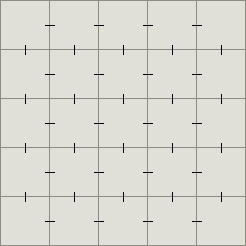
\includegraphics[width=\textwidth,height=1.14583in]{map-as-graph.png}
\caption{Map as graph}
\end{figure}

Example:
\url{https://www.redblobgames.com/pathfinding/grids/graphs.html\#grids}

\end{frame}

\begin{frame}{Dijkstra's Algorithm}
\protect\hypertarget{dijkstras-algorithm}{}

Dijkstra's Algorithm works by visiting vertices in the graph starting
with the object's starting point. It then repeatedly examines the
closest not-yet-examined vertex, adding its vertices to the set of
vertices to be examined.

\begin{figure}
\centering
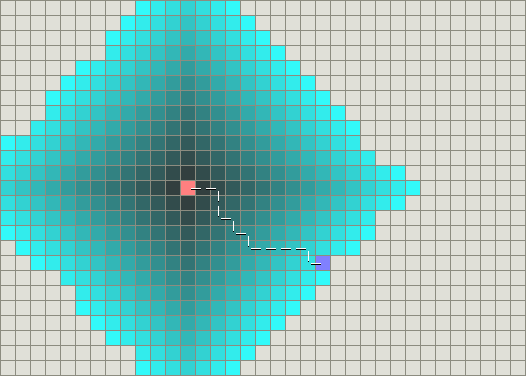
\includegraphics[width=\textwidth,height=1.5625in]{dijkstra.png}
\caption{Dijkstra algorithm}
\end{figure}

\end{frame}

\begin{frame}{Gready Best-First search}
\protect\hypertarget{gready-best-first-search}{}

The Greedy Best-First-Search algorithm works in a similar way, except
that it has some estimate (called a heuristic) of how far from the goal
any vertex is. Instead of selecting the vertex closest to the starting
point, it selects the vertex closest to the goal. Greedy
Best-First-Search is not guaranteed to find a shortest path.

\begin{figure}
\centering
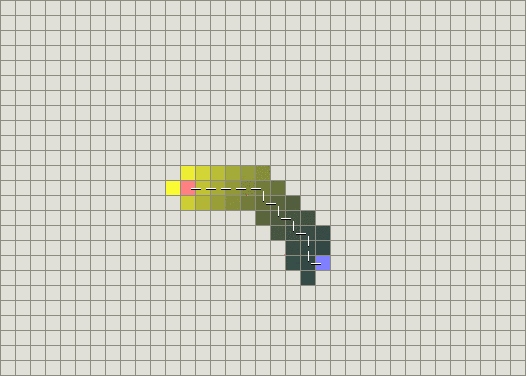
\includegraphics[width=\textwidth,height=1.33333in]{best-first-search.png}
\caption{Greedy Best-first search}
\end{figure}

\end{frame}

\begin{frame}{Dijkstra's Algorithm and Best-First-Search}
\protect\hypertarget{dijkstras-algorithm-and-best-first-search}{}

Let's consider the concave obstacle as described in the previous
section. Dijkstra's Algorithm works harder but is guaranteed to find a
shortest path:

\begin{figure}
\centering
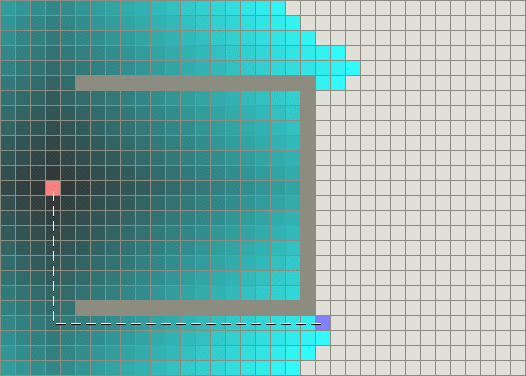
\includegraphics[width=\textwidth,height=1.5625in]{dijkstra-trap.png}
\caption{Dijkstra's Algorithm with obstacle}
\end{figure}

\end{frame}

\begin{frame}{Dijkstra's Algorithm and Best-First-Search}
\protect\hypertarget{dijkstras-algorithm-and-best-first-search-1}{}

Greedy Best-First-Search on the other hand does less work but its path
is clearly not as good:

\begin{figure}
\centering
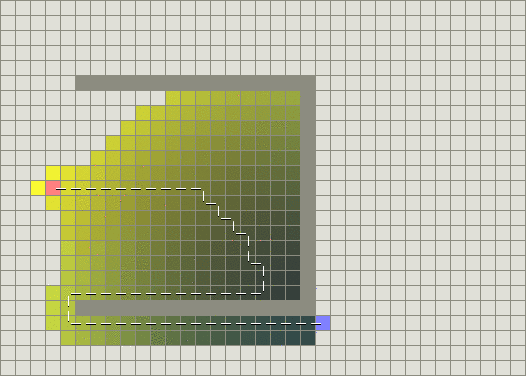
\includegraphics[width=\textwidth,height=1.5625in]{best-first-search-trap.png}
\caption{Greedy Best-First Search with trap}
\end{figure}

\end{frame}

\begin{frame}{The A* Algorithm}
\protect\hypertarget{the-a-algorithm}{}

A* is like Dijkstra's Algorithm in that it can be used to find a
shortest path. A* is like Greedy Best-First-Search in that it can use a
heuristic to guide itself. In the simple case, it is as fast as Greedy
Best-First-Search:

\begin{figure}
\centering
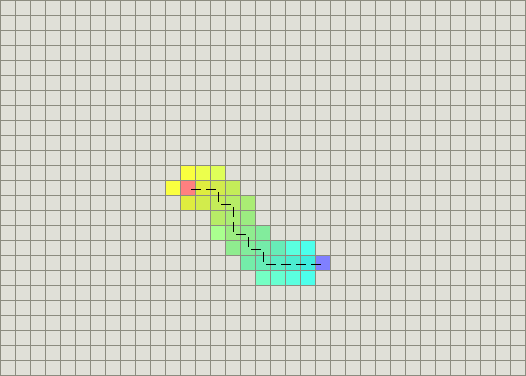
\includegraphics[width=\textwidth,height=1.5625in]{a-star.png}
\caption{A* algorithm}
\end{figure}

\end{frame}

\begin{frame}{References}
\protect\hypertarget{references}{}

\begin{itemize}
\tightlist
\item
  https://en.wikipedia.org/wiki/A*\_search\_algorithm
\item
  http://theory.stanford.edu/\textasciitilde{}amitp/GameProgramming/AStarComparison.html
\end{itemize}

\end{frame}

\end{document}
